\documentclass[iutinfo,a4paper,nocorrections,10pt]{ustl-tdtp}
%\usepackage[utf8]{inputenc}
%\usepackage[a4paper]{geometry}

\etablissement{\ustl}
\formation{DUT info 2ème année}
\matiere{Structures de données}
\titre{TP 2 : Listes}
\date{\annee{2018}--\annee{2019}}

\parindent 0cm
\begin{document}
\maketitle
\thispagestyle{empty}


%\section{}
\sloppy
\section{Utilisation de l'interface List}

Dans une classe ListUtils, en utilisant l'une des implémentations de l'interface Java List, on vous demande de:
\begin{enumerate}
\item Créer une méthode \texttt{List<Integer> genereRdmIntList} qui génère une liste d'entiers de taille aléatoire (30 maximum tout de même!), initialisée avec des entiers positifs tirés aléatoirement et inférieurs à 100.

\item Écrire une méthode \texttt{affiche(List<Integer> l)} pour pouvoir afficher la liste sous la forme:\\
$a \rightarrow b \rightarrow ...\rightarrow x$, où a est la valeur du premier entier de la liste, b la seconde, et ainsi de suite. Pour ce faire, vous utiliserez un itérateur. N'oubliez pas le retour à la ligne.

\item Écrire une méthode \texttt{afficheInverse(List<Integer> l)} qui affiche la liste en ordre inverse. Vous utiliserez cette fois-ci un itérateur de type \texttt{ListIterator} qui permet d'itérer sur une liste dans les deux sens(cf. Javadoc). N'oubliez pas le retour à la ligne.

\item Écrire une méthode \texttt{int somme(List<Integer> l)} qui renvoie la somme des éléments de la liste.
\item Écrire une méthode \texttt{int moyenne(List<Integer> l)} qui renvoie la moyenne entière des éléments de la liste.
%\item Ecrire une méthode \texttt{position(int i)} qui, étant donné un entier, renvoie la position de sa premiére occurence dans la liste ou ?1 si il n?y est pas.
\item Écrire une méthode \texttt{int max(List<Integer> l)} qui retourne la valeur maximale contenue dans la liste.
\item Écrire une méthode \texttt{int min(List<Integer> l)} qui renvoie la valeur minimale contenue dans la liste.
\item Écrire une méthode \texttt{List<Integer> positions(List<Integer> l, int n)} qui, étant donné un entier $n$, renvoie la liste des positions (renvoie la liste vide sinon).\\
Exemple :$1 \rightarrow 22 \rightarrow 45 \rightarrow 56 \rightarrow 1 \rightarrow 34 \rightarrow 1$\\
\texttt{positions(1)} doit renvoyer $0 \rightarrow 4 \rightarrow 6$
\item Écrire une méthode \texttt{List<Integer> paire(List<Integer> l)} qui renvoie la liste des éléments pairs.
\item Écrire une méthode \texttt{boolean estTrie(List<Integer> l)} permettant de vérifier si la liste est triée dans l'ordre croissant.
\item Écrire une méthode \texttt{List<Integer> trie(List<Integer> l)} qui renvoie une liste triée (on pourra s'aider de certaines des méthodes précédentes).
\end{enumerate}

\textbf{En utilisant le framework JUnit et la classe \texttt{ListUtilsTest} fournie dans les ressources du TP, assurez-vous que toutes vos méthodes passent les tests associés avant de passer à la suite. Vos classes de test seront placés dans un répertoire de sources \texttt{tests}.}

\section{Implémentation d'une liste simplement chaînée à double extrémité}

Dans cette partie, nous allons réaliser l'implémentation d'une liste simplement chaînée à double extrémité. Comme indiqué sur la Figure~\ref{fig:double-ended}, il s'agit d'une liste simplement chaînée qui dispose d'un lien supplémentaire vers le dernier élément. 

\begin{figure}[!h]
\centering
\label{tableau}
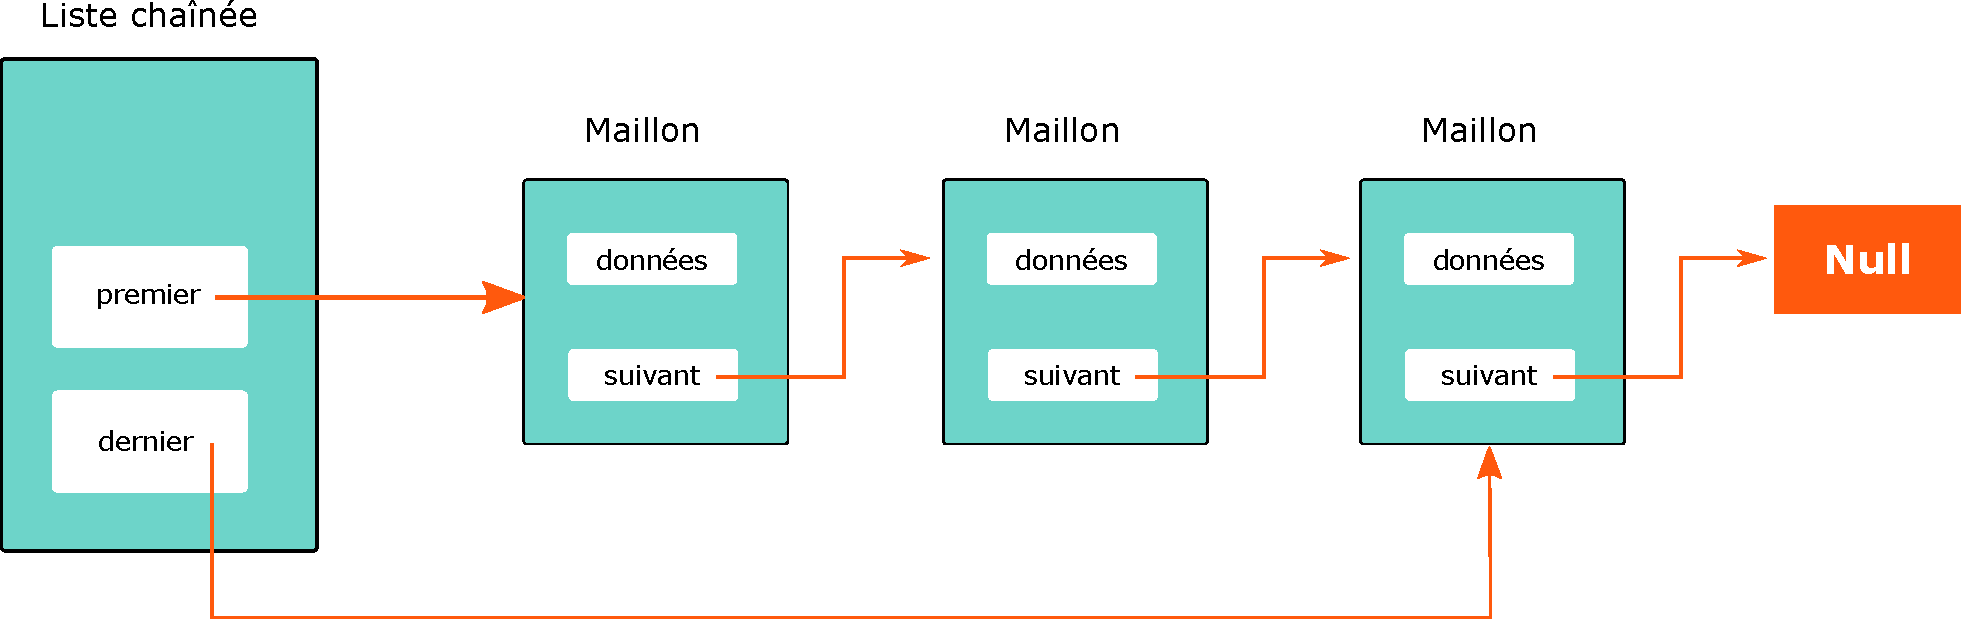
\includegraphics[scale=0.5]{figs/linked_list_double_ended}
\caption{Liste à double extrémité}
\label{fig:double-ended}
\end{figure}

Nous utiliserons la représentation suivante: une liste contient les références sur le premier noeud et sur le dernier noeud, chaque noeud contient une valeur et une référence vers le noeud suivant. 
~\\
	\texttt{public class MyList<E>} \{
	\begin{description}
		\item \texttt{Node<E> first;}
		\item \texttt{Node<E> last;}


		\item // méthodes pour traiter une liste
		\end{description}
	\}
	

%\item Noeud contenant un int:\\
	\texttt{public class Node<E> 
	\{ }
	\begin{description}
	
	\item	\texttt{E value;}
\item		\texttt{Node<E> next;}
\end{description}
	
\vdots

		
\}
~\\
		
		
Pour connaître le comportement des méthodes suivantes à implémenter, vous vous appuierez sur la Javadoc de l'interface List.

~\\ \textbf{Question 1 :} Créez une classe \texttt{Node<E>} qui
contiendra la référence sur l'objet qu'il contient (la valeur de l'élément) et aussi la
référence sur l'objet de type \texttt{Node<E>} successeur. Créez aussi
le constructeur.

~\\ \textbf{Question 2 :} Créez une classe \texttt{MyList<E>}. Créez et implémentez le constructeur sans paramètre de \texttt{MyList<E>}.

~\\ \textbf{Question 3 :} Programmez les méthodes :
\begin{verbatim}
  boolean add(E e) 
  String toString() /*Renvoie une chaîne de caractères contenant
   les éléments de la liste séparés par des virgules,
   et encadrée pas des crochets.*/ 
  boolean isEmpty()
  int size()
  void clear()
  E get(int index)
\end{verbatim}

~\\ \textbf{Question 4 :} Programmez les méthodes suivantes de recherche dans la
liste:
\begin{verbatim}
 int indexOf(Object o) 
 boolean contains(Object o) 
 int lastIndexOf(Object o) 
\end{verbatim}


~\\ \textbf{Question 6 :} Programmez les méthodes suivantes d'ajout et de suppression dans la liste:
\begin{verbatim}
 void add(int index, E element) 
 E remove(int index)//Supprime l'élément situé à l'indice index et le retourne.
 boolean remove(Object o) 

\end{verbatim}
\textbf{En utilisant le framework JUnit et la classe \texttt{MyListTest} fournie dans les ressources du TP, assurez-vous que toutes vos méthodes passent les tests associés.}

\section{Implémentation d'une liste doublement chaînée}

\textbf{Question 7 :} Créez une classe \texttt{MyDoubleList<E>}. Cette classe reprend les mêmes méthodes que la classe \texttt{MyList}. Vous ajouterez à l'objet \texttt{Node} un attribut qui référence le maillon précédent, de manière à implémenter une liste doublement chaînée. Modifiez vos méthodes en conséquence en veillant à tirer partie de l'avantage conféré par cette nouvelle implémentation.


\end{document}
